\documentclass[11pt]{article}
\usepackage[utf8]{inputenc}
\usepackage{amsmath}
\usepackage{amssymb,amsfonts,latexsym,cancel}
\usepackage{graphicx}
\usepackage{epstopdf}
\usepackage{tabularx} 
\usepackage{float}
\usepackage{verbatim}
\usepackage[left=2cm, right=2cm, top=2cm, bottom=2cm]{geometry}
\setlength\parindent{0pt}
\setlength{\parskip}{2mm}

\title{MultiFEBE \\ME-ST-SR-004 [TUTORIAL] \\ \textbf{Spherical Shell (FEM model)}}
\author{Samuel González-Jiménez and Jacob D. R. Bordón}
\date{September 2025}

\begin{document}
	\maketitle
	
	\section*{Problem description}
	In this validation case a static analysis of the Spherical shell problem \cite{MacNeal1985} is performed using the Finite Element Method. As shown in Figure \ref{Sph_draw} the problem consist on a quarter of a spherical shell of 10.0 in radio and a thickness of 0.04 in with a hole in the top. The properties of the material are a Young modulus (E) of $6.825 \times 10^{7}  \ \text{lbf}/\text{in}^2$ and a Poisson ratio ($\nu$) of 0.3. The concentrated forces (in in) and the boundary supports are displayed in Figure \ref{Sph_draw}. The mesh is $N \times N$ on quadrant.
	
	\begin{figure}[H]
		\centering
		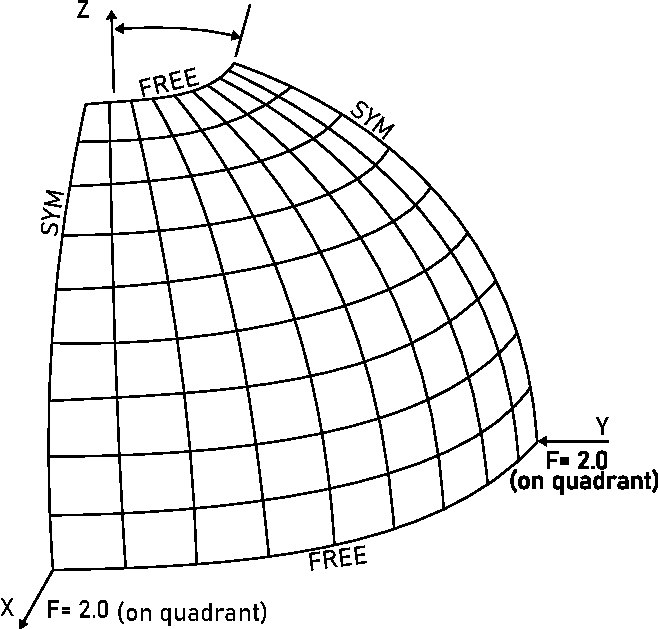
\includegraphics[scale=0.60]{Spherical_dome_draw.pdf}
		\caption{Scordelis-Lo roof problem}
		\label{Sph_draw}
	\end{figure}
		
	
	\section*{Input data file}
	In this section, the principal block sections of the MultiFEBE input data file will be reviewed.
	The first block to be dealt is the settings one. In this case the mesh is imported from another file named \texttt{"spherical\_dome.msh"} in the Gmsh MSH format version 2.2.
	
	\begin{verbatim}
	[settings]
	mesh_file_mode = 2 "spherical_dome.msh"}
	\end{verbatim}
	
	In the section [symmetry], two planes of symmetry are defined, since only a quarter of the problem is meshed, as shown in Figure \ref{Sph_draw}. To the correct recognition of the symmetry planes, each axis of symmetry must intersect the origin of coordinates.
	
	\begin{verbatim}
	[symmetry planes]
	plane_n1: symmetry
	plane_n2: symmetry
	\end{verbatim}
					
	In the section [export], it is defined that only the nodal solutions for node 1 were displayed, which is where the load is applied on the X-axis and where the convergence study will be performed.
		
	\begin{verbatim}
	[export]
	nso_nodes= 1, 1
	\end{verbatim}
	
	Since the problem is solved with Shell finite elements, in the [cross sections] section are defined the number of fe subregions related to the cross section (1), fe subregion identifier (1), type of cross section (degshell), thickness (0.04) and reference vector for x' direction (0. 0. 1.).
	
	\begin{verbatim}
	[cross sections]
	1
	degshell 1 1 0.04d0 0. 0. 1.
	\end{verbatim}
	
	In the [groups] section, 2 groups are defined. The group 1 selects the node in X-axis where the force is applied, and group 2 does the same but for the node in the Y-axis.
	
	\begin{verbatim}
	[groups]
	2
	1 nodes ball interior 10.d0  0. 0. 0.01d0 1
	2 nodes ball interior  0. 10.d0 0. 0.01d0 1
	\end{verbatim}
	
	Finally in [conditions over nodes] section, the loads are applied in their respective axes. Note that the force is half that applied in the problem, since due to symmetry, the corresponding node has only half the stiffness of the entire problem. Furthermore, movement in Z is restricted in group 1, since otherwise the spherical shell would move along that axis.
	
	\begin{verbatim}
	[conditions over nodes]
	group 1: 1 1.d0
	         0 0
	         0 0
	         0 0
	         1 0
	         0 0

	group 2: 0 0
	         1 -1.d0
	         1 0
	         1 0
	         0 0
	         0 0
	\end{verbatim}

	\section*{Results and discussion}
	
	In this section the results for the convergence of an NxN study is shown. In total 20 meshes were tested, with 2, 4, 8 and 16 elements and 5 different types of elements, i.e. MITC3i, MITC6a, MITC8* and MITC9 (see~\cite{Bathe2006}). The characteristics of each type of element is shown in Table \ref{MITC_tab}.
	
	\begin{table}[H]
	\caption{Element types characteristics}
	\label{MITC_tab}
	\centering
	\begin{tabular}{|c|c|c|}
		\hline
		\textbf{Element} & \textbf{Element shape} & \textbf{Order} \\
		\hline
		MITC3i & Triangular & Linear \\
		\hline
		MITC6a & Triangular & Quadratic \\
		\hline
		MITC4 & Quadrilateral & Linear \\
		\hline
		MITC8* & Quadrilateral & Quadratic \\
		\hline
		MITC9 & Quadrilateral & Quadratic \\
		\hline
	\end{tabular}
	\end{table}
	
	Figure \ref{ux} shows the convergence to X-axis displacement at the node where the X-axis load is applied (node 1), to the theoretical result of 0.0940 inch for each element type according to the number of elements.
	
	\begin{figure}[H]
		\centering
		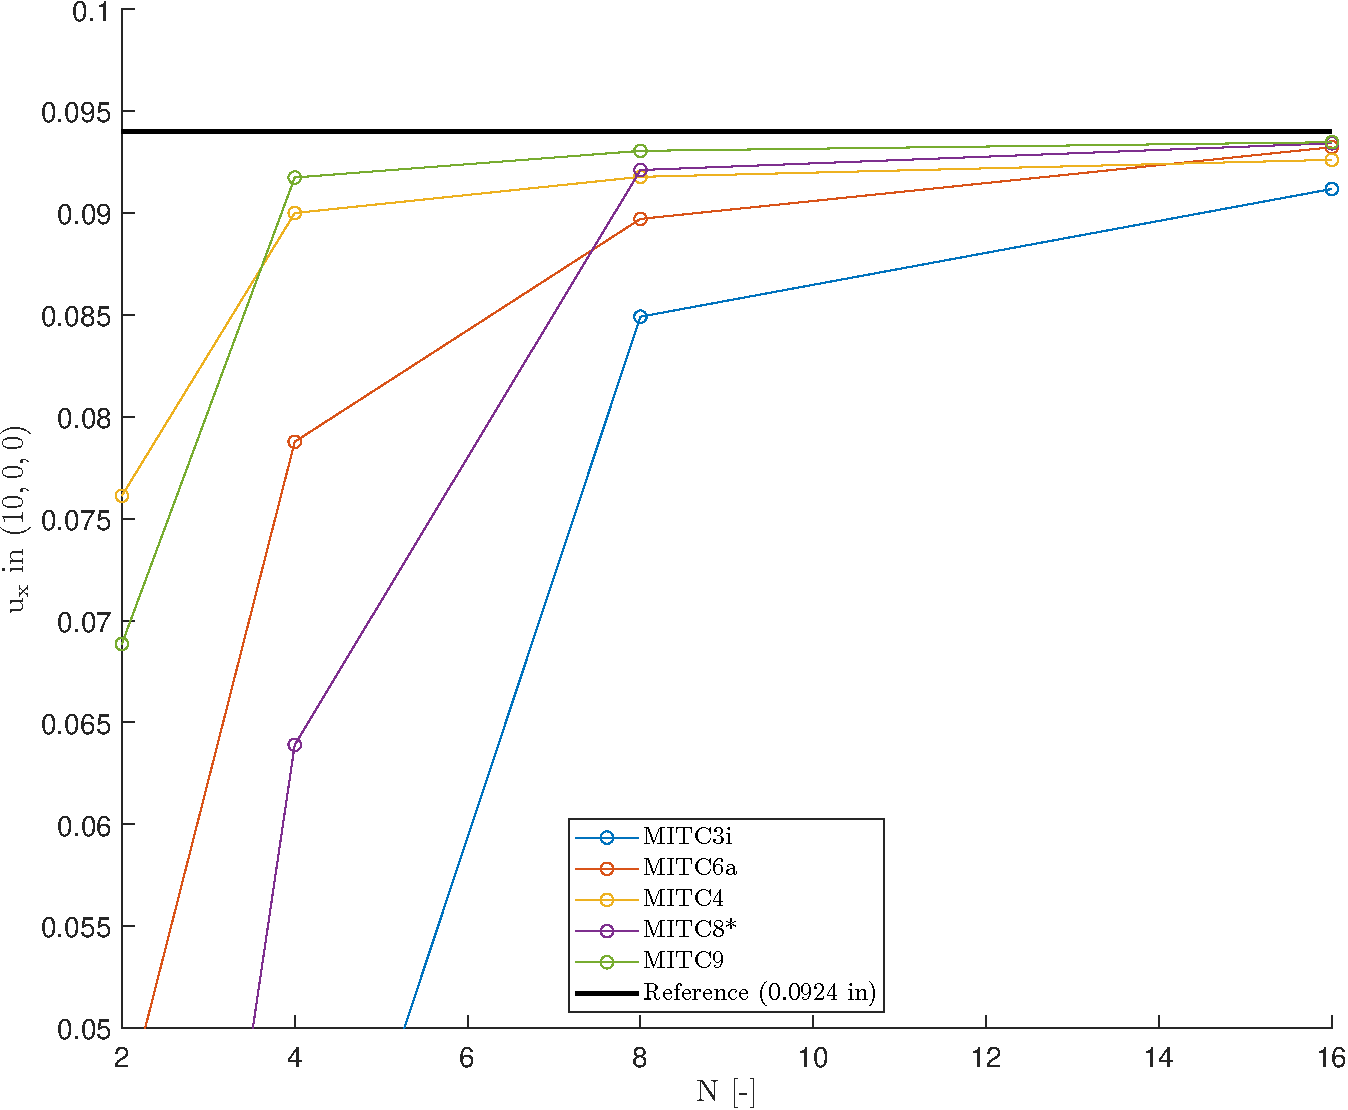
\includegraphics[scale=0.55]{ux_at_load.pdf}
		\caption{X-axis displacement at node 1 study.}
		\label{ux}
	\end{figure}
	
	Except for case MITC3i, convergence is slightly below the reference result, with a faster convergence in cases MITC4 and MITC9.
	
	Figure~\ref{deformed_shape} shows the deformed shape of the meshed spherical shell visualized in Gmsh from the .pos file.
	
	\begin{figure}[H]
		\centering
		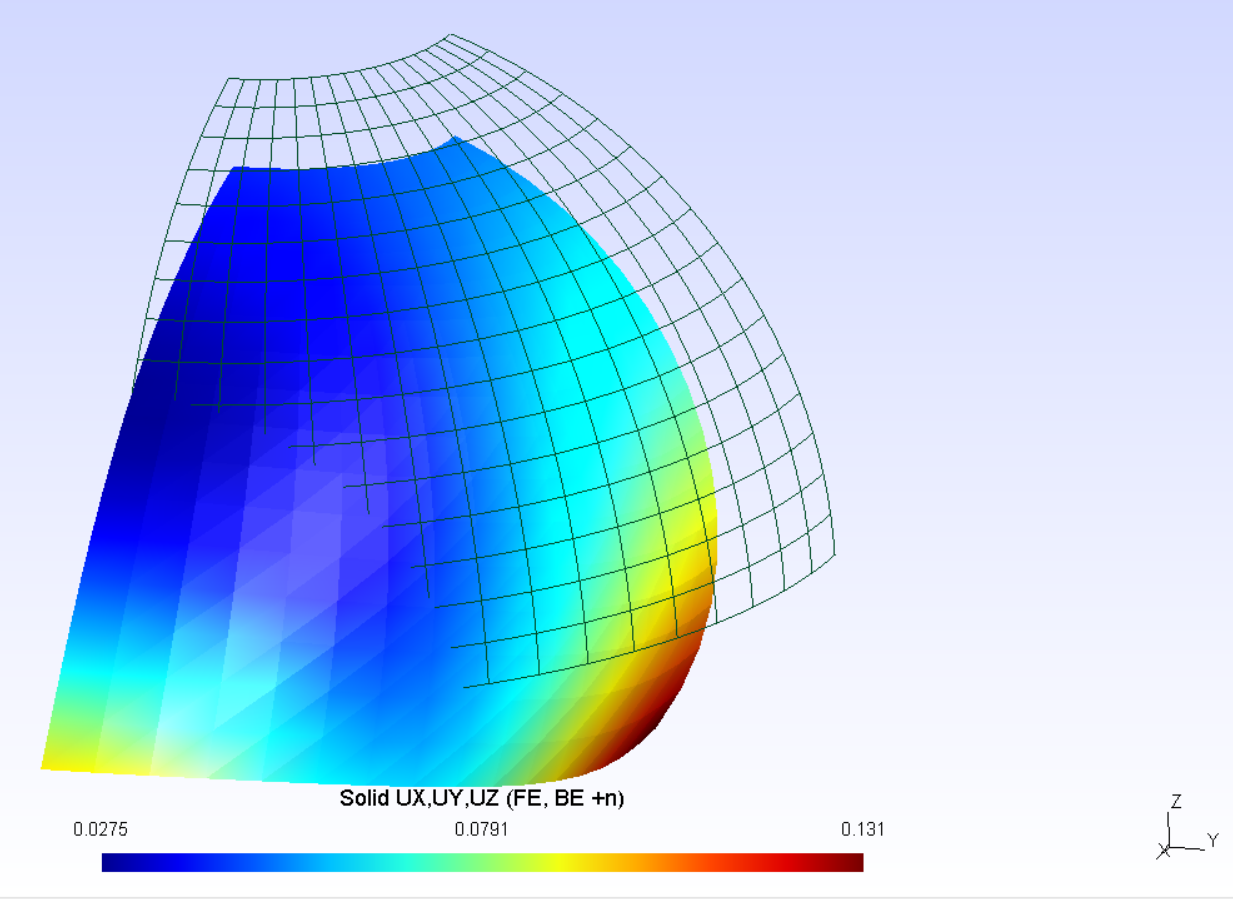
\includegraphics[scale=0.40]{Spherical-dome deformed shape}
		\caption{Deformed shape of the quarter of spherical shell for the MITC9 case.}
		\label{deformed_shape}
	\end{figure}
	
	\section*{Attachments}
	 
	 For this validation case, the convergence study execution file is attached as well as the .dat, .mesh and the .geo file. 	 
	 
	 \bibliographystyle{unsrt}
	 \bibliography{references.bib}
	 
	 \end{document}